% !TeX root = ../../main.tex
% chktex-file 24
\section{Ubi-Interact}\label{section:ubi-interact}

\ac{UBII} is a framework for distributed applications, which enables to connect all kinds of different devices together. A centralized server is used to manage the system in a local network. It is currently developed and maintained by Sandro Weber, who is also the advisor for this thesis. The abstraction into devices, topics and interactions allows to decouple the implementation of a software from device specific environments.


\subsection{Architecture}\label{subsection:architecture}

The main components of the \ac{UBII} framework are:
\begin{description}
	\item[Clients] describe a basic network participant. For every client registered in the system, exists one network socket adress. So clients are an abstraction of a physical network device. They are defined by a unique identifier. 
	\item[Devices] can be registered by clients. A device is an abstraction for a virtual device, which groups different input and output devices together. It is defined by a unique identifier and a list of components.
  \item[Components] contain the topic name, message format for input/output devices and wether it publishes input or receives output data. A data source for such an input device, could be any sensor for example a button or an \ac{IMU}. Data output examples for input devices are lamps and displays.
  \item[Message Formats] are strings which identify a certain data format. Most common data types are available, like for example \textit{Vector4\( \times \)4}, \textit{Vector2} or \textit{Vector3}.
	\item[Topics] are data channels which are addressed by a name. Clients can publish messages to topics, which are registered by a device. Clients are also able to receive messages, after subscribing to a topic. Such messages (also called \enquote{topic data}) are formatted as JSON\footnote{JSON is a standardized data exchange format, that uses human-readable text. It is often used for web-based data communication.}-string, whose structure is defined by the device.
	\item[Sessions] operate on the server, but can be specified by the client. They are defined by a unique identifier as well as a list of interactions and \textbf{input/output mappings}. The mappings are defined by a message format and topic name.
	\item[Interactions] are reactive components. They operate on topics and are defined by a source code snippet\footnote{Currently only JavaScript is supported as a script language.}. Interactions are executed in a fixed interval on the \ac{UBII} server. They can subscribe to topics and use the received topic data as input, given an input/output mapping description. The output of the interaction is published into another topic. It is also possible to keep data to use in future executions (persistent state).
\end{description}

\begin{figure}[htpb]
  \centering
  \begin{subfigure}{.5\textwidth}
    \centering
    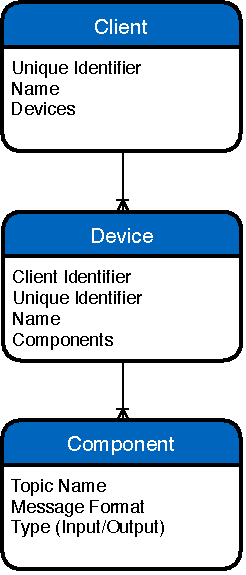
\includegraphics[width=3cm]{figures/ubii_er_client.pdf}
    \caption{The client components.}\label{fig:ubii_er_client}
  \end{subfigure}%
  \begin{subfigure}{.5\textwidth}
    \centering
    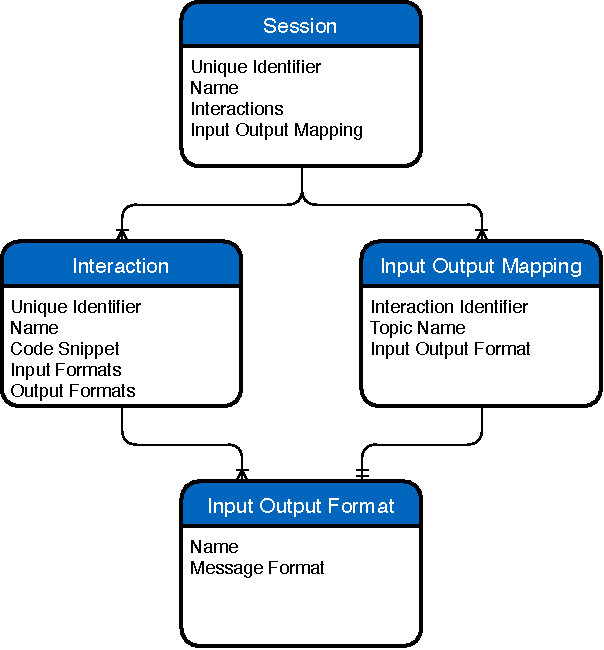
\includegraphics[width=7cm]{figures/ubii_er_server.pdf}
    \caption{The session components.}\label{fig:ubii_er_server}
  \end{subfigure}
  \caption[UBII Components Diagram]{Relationships of the core components in an entity relationship diagram.}\label{fig:ubii_er}
\end{figure}


\subsection{Interactions}\label{subsection:interactions}
An powerful but optional core feature of \ac{UBII} are so called interactions. As explained in the component overview~(see~\ref{subsection:architecture}), they are reactive components, which operate on topics and regularly execute given code snippets (processing functions) on the \ac{UBII} server. Interactions are isolated components, which just depend on topic data and nothing else. This abstraction introduces the possibility to reuse logic in other applications in similar context. 

\begin{figure}[htpb]
  \centering
  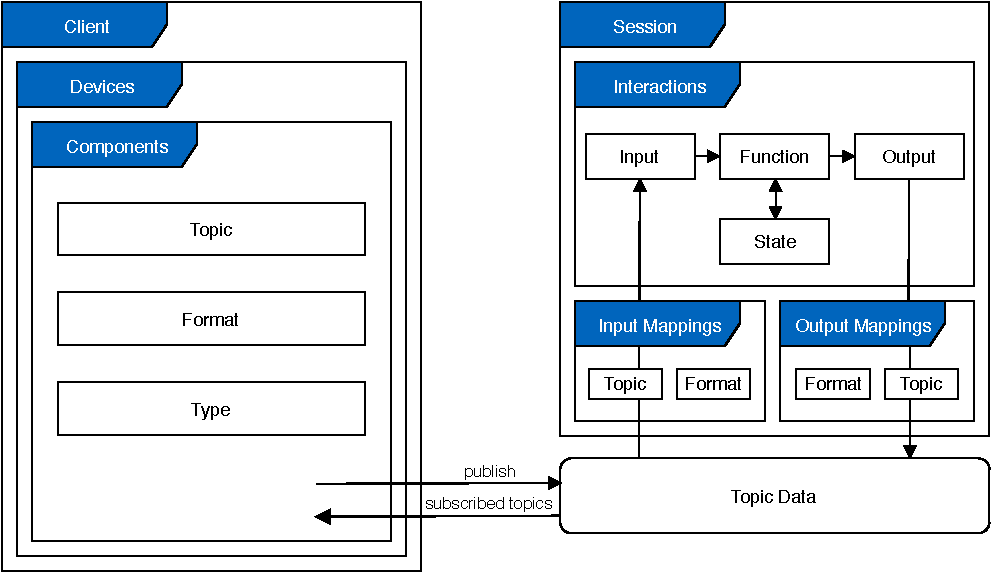
\includegraphics[width=12cm]{figures/ubii_cd.pdf}
  \caption[UBII Communication Diagram]{Interaction processing overview. This graphic gives a rough overview of the dataflow when using an interaction. Conceptualized with the help of Sandro Weber.}\label{fig:ubii_cd}
\end{figure}

The code snippet has to define a function, which accepts three parameters: 
\lstinline{inputs} is a collection of values, which were published into a topic. The topic which was used, is defined by the input mappings of the session. \lstinline{outputs} is an empty collection, where values can be added. Those values are then published into a topic, defined by the output mappings of the session. \lstinline{state} stores a persistent collection of values, which can be used in later executions of the same interaction.

\begin{figure}[htpb]
  \centering
  \begin{tabular}{c}
  \begin{lstlisting}[language=JavaScript]
    // detect intentional movement by comparing the current position with a previous one
    function (inputs, outputs, state) {
      const threshold = 0.05;

      if (state.position) {
        const vector = {
          x: inputs.position.x - state.lastPosition.x,
          y: inputs.position.y - state.lastPosition.y,
        };
  
        const squaredDistance = Math.pow(vector.x, 2) + Math.pow(vector.y, 2);
  
        outputs.moved = squaredDistance < threshold;
      } else {
        outputs.moved = true;
      }

      state.lastPosition = inputs.position;
    }
  \end{lstlisting}
  \end{tabular}
  \caption[A basic UBII interaction in JavaScript.]{An example for an interaction written in JavaScript. This interaction calculates the squared distance of two points. One of the points comes from the input, while the other one is stored in the state. To achieve this, the euclidean vector norm of the subtraction of both vectors without the square root is calculated and compared with a threshold constant. The result is then written into the output as a boolean data type.}\label{fig:ubii_interaction_example}
\end{figure}

Interactions should be designed generalized, so that they are easy to reuse. They can be used to discretize data, converting data to other formats or just to outsource some logic from the application. Concrete examples include detecting button presses, changing coordinate spaces and evaluate data.
% this might be left out or merged into above
They are also useful, if you want to connect two topics with different formats. Imagine an application, which consumes a rotation given in euler angles in radians. But some devices publish euler angles in degrees. We could implement an interaction, which takes euler angles in degrees from one topic and publishes euler angles in radians to another one, which then is used by the application.
